\thispagestyle{endchapter}

\begin{tcolorbox}

\vspace{80pt}
	\lettrine{A}{bsolutely} brilliant expedition: pity it had to end after 4 weeks! The elusive connection to form the second-longest cave in Slovenia is still being sought, though we're down to 28 m separation (with a survey error of \textasciitilde 40 m) in an absolute maze of corridors and drops.
 
 Most of all, this expedition was an enormous training mission: we now have an extremely strong expedition team together once more, with great ties to the new JSPDT members.

All the lags can feel extremely proud of the enormous
cannon of information that has been passed on, the new members proud of the steep learning curve that they all conquered, and everyone proud of the Caves, little and big, deep and shallow that we've found this year.
 
    How to explain expedition fever? The call of the unknown, the burning desire to stand once again on the pushing front\ldots{} stumbling home from a caving trip over the moonscape of the plateau to greet the warm glow of the fire in the Bivvi\ldots{} the ring of the hammer as you place the bolts to abseil down a new pit\ldots{} the solitude of climbing in darkness, the warm glow of humanity when returned to your company\ldots{} But such concerns do not convince your supervisor or bank manager to elope for 5 whole weeks.

    So, to speak objectively, we have the genuine possibility of connecting \passage{Vrtnarija} to \passage{Sistem Migovec} and forming the 2\(^{nd}\) longest cave in Slovenia (\passage{Postojna}, number 1 slot, can only be fully explored by cave diving). The distance between \passage{Vrtnarija} and \passage{M2} (\passage{Sistem Migovec}) was closed to 30 m at closest approach by the end of 2007 (error guessed at circa. 50 m). We have a mountain that sits on the watershed between the Adriatic and Black Sea, with possibly the most complicated alpine speleogenesis in the world, and a whole host of secrets to unlock. We have new caves descending into blank mountain, and deep leads near the bottom of \passage{Vrtnarija} that must be pushed soon before the decay of the bolts puts them beyond reach.

    The controls are set for the heart of the hollow mountain.



\end{tcolorbox} 
	\backgroundsetup{	scale=1.1,
					color=black,
					opacity=1,
					angle=0,
					contents={%
							  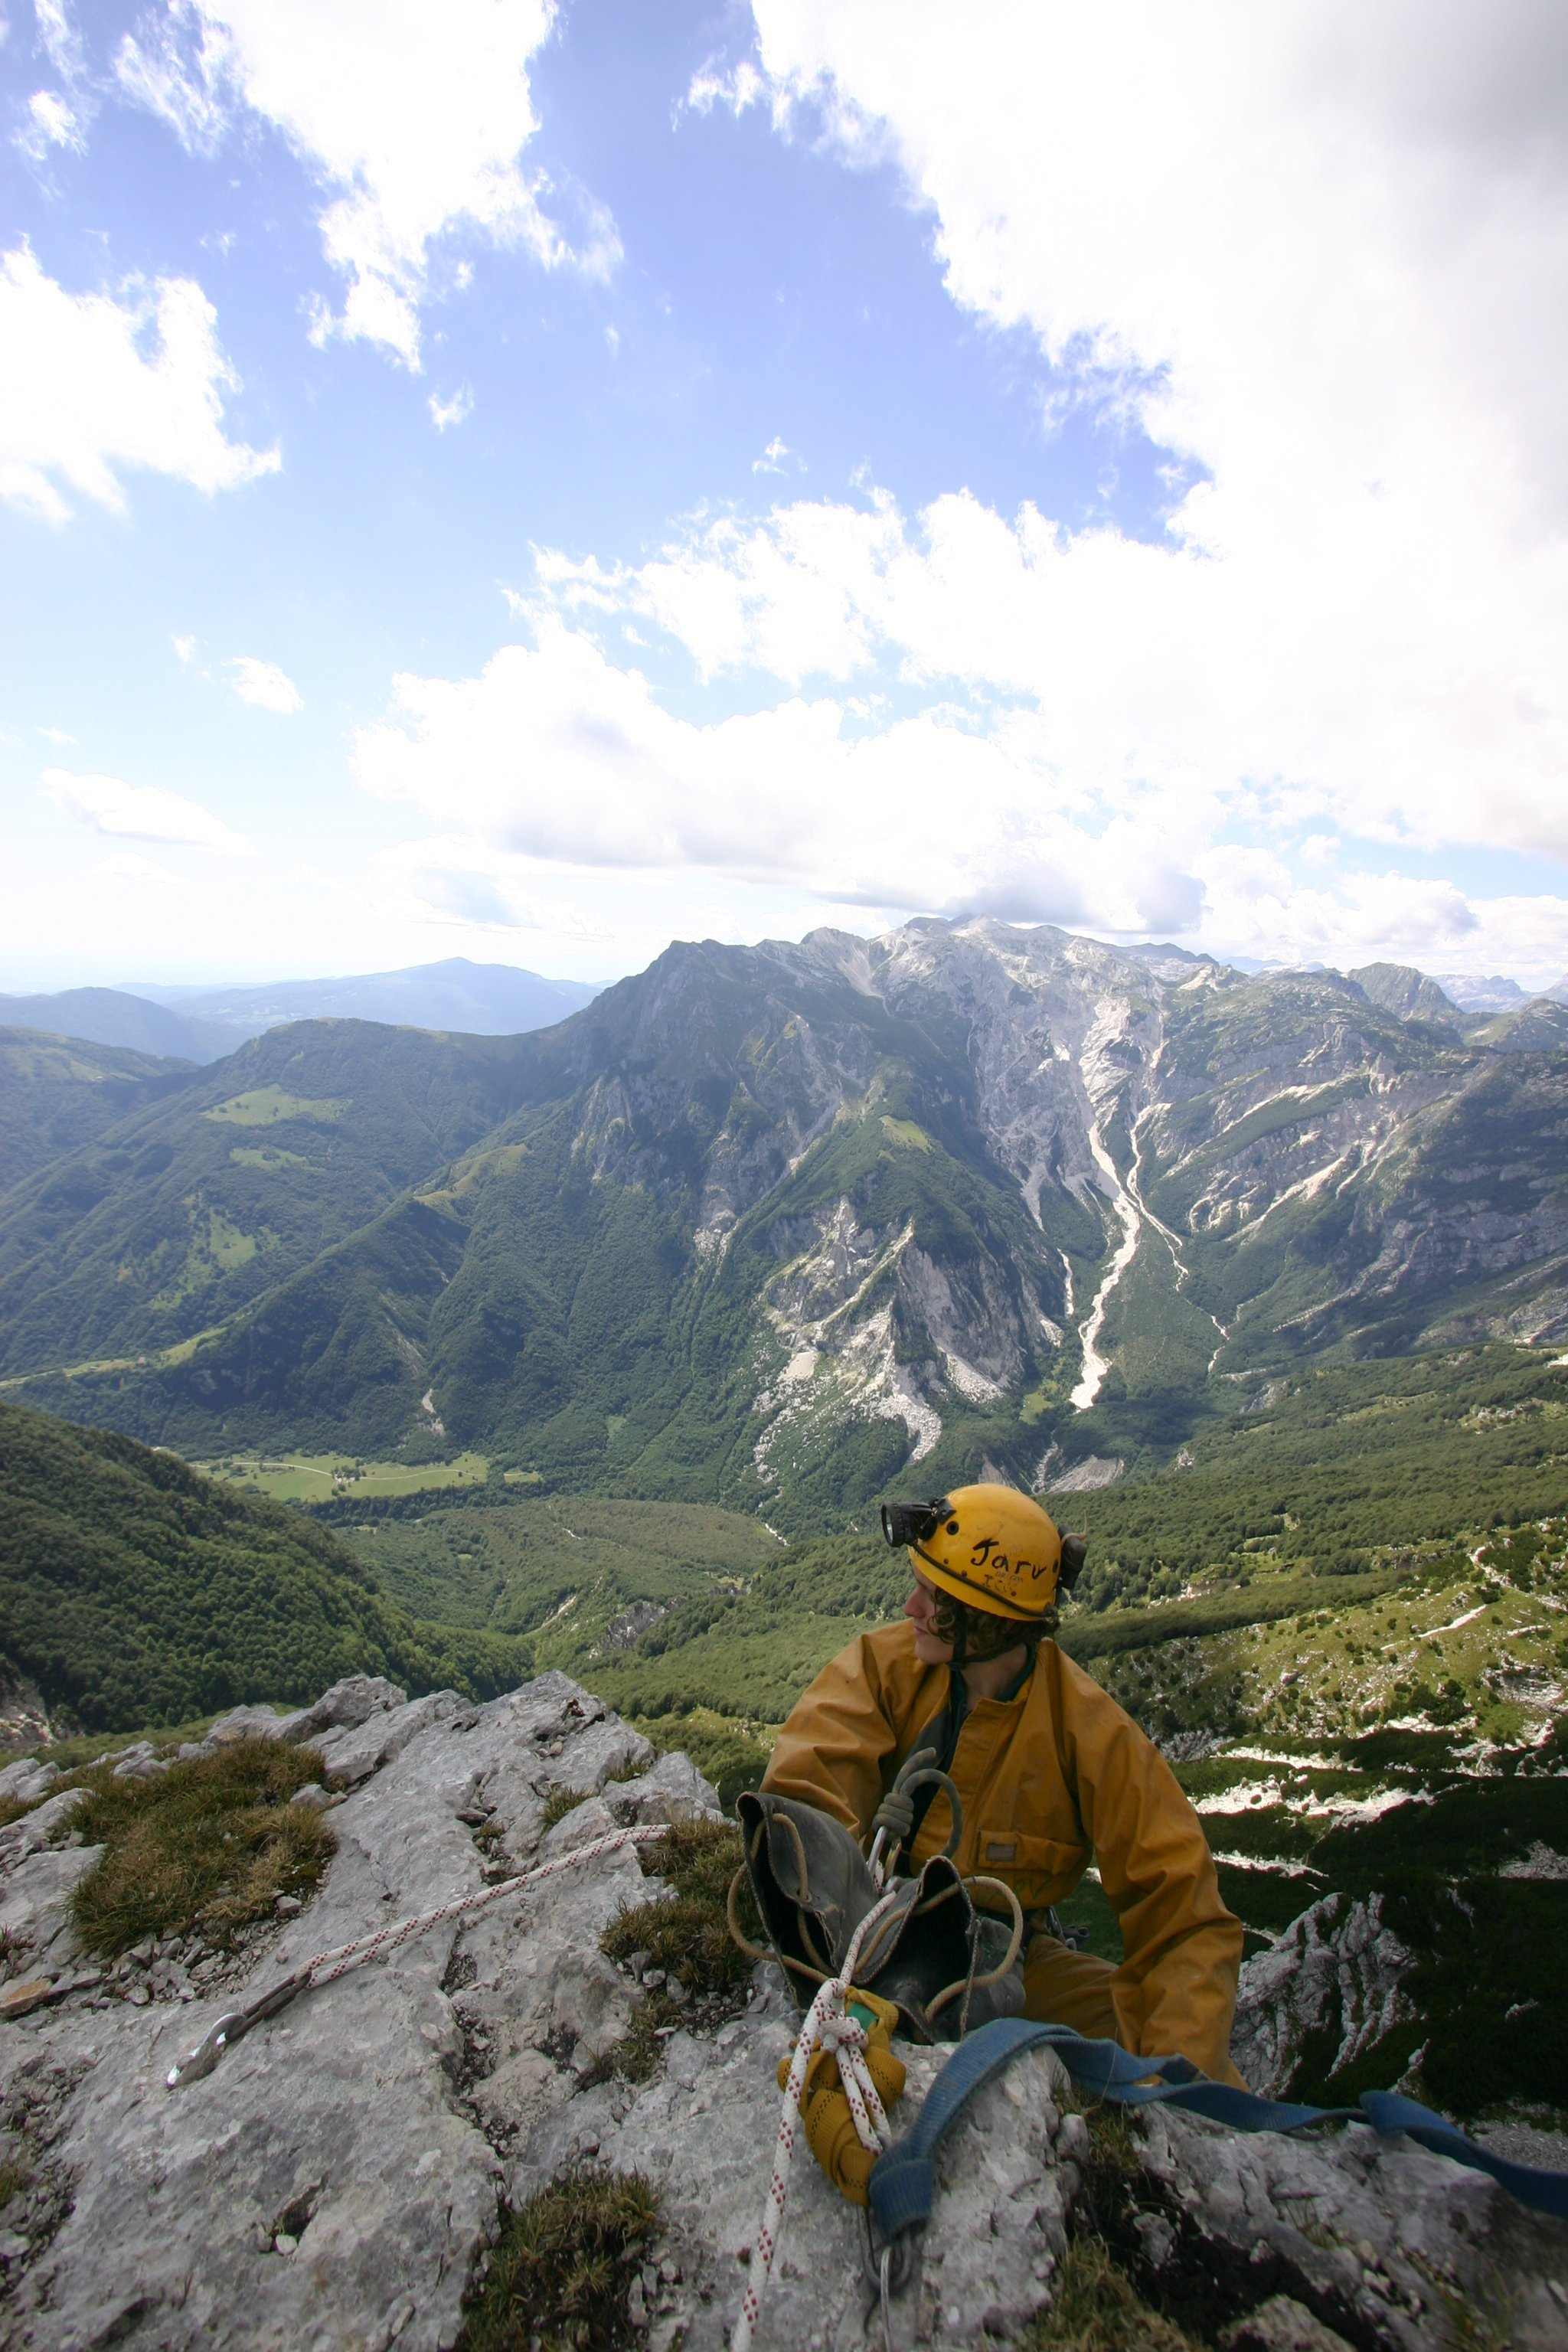
\includegraphics[height=\paperheight]{2007/outro/martin mcgowan -jarvist hawk cave abseil--orig.jpg}
 					}
	}
\BgThispage
